%%%%%%%%%%%%%%%%%%%%%%%%%%%%%%%%%%%%%%%%%%%%%%%%%%%%%%%%%%%%%%%%%%%%%%%%
% Plantilla TFG/TFM
% Escuela Politécnica Superior de la Universidad de Alicante
% Realizado por: Jose Manuel Requena Plens
% Contacto: info@jmrplens.com / Telegram:@jmrplens
%%%%%%%%%%%%%%%%%%%%%%%%%%%%%%%%%%%%%%%%%%%%%%%%%%%%%%%%%%%%%%%%%%%%%%%%

\chapter{Marco Teórico}
\label{marcoteorico} 

\section{Estudio del mercado}
Antes de empezar con el desarrollo del proyecto es importante un estudio de las alternativas en el mercado y entender el objetivo de este trabajo.

\subsection{Bcoach}
Esta aplicación ofrece la opción de crear equipos personalizados y con cada uno realizar una tarea planificada animada con elementos gráficos para que sea fácilmente visualizable. Ofrece 3 planes con más o menos funcionalidades para el entrenador:

\subparagraph{Bcoach - Licencia Tablet/Ipad (2,99€/mes)}
Este es el plan más sencillo, incluye gestión de entrenamientos; pizarra táctica; estadísticas de partidos y la app estará disponible en cualquier dispositivo Tablet/iPad. Toda la información será almacenada de manera local en un solo dispositivo.

\subparagraph{Bcoach Cloud - Licencia Multiplataforma (5,99€/mes)}
Este plan incluye todo lo anterior, además de que la información estará sincronizada en la nube y ofrece acceso a Bcoach web.

\subparagraph{Bcoach Pro - Licencia + Asesoramiento(299,99€/mes)}
Esta licencia es la más completa de todas, ofreciendo adicionalmente asesoramiento deportivo.

\begin{figure}[H]
    \centering
    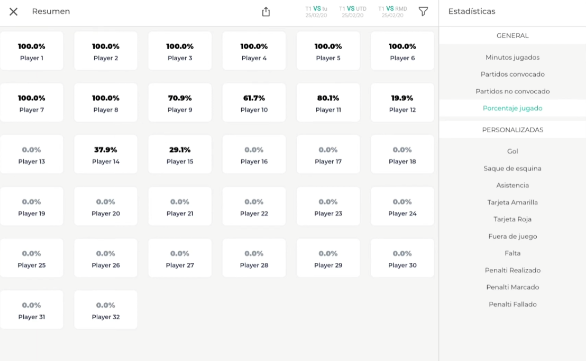
\includegraphics[width=10cm]{archivos/tfg_jorge/bcoach_ests_jugadores}
    \caption{Bcoach - Estadísticas de Jugadores}\label{sistemass2}
\end{figure}

\subsubsection{Manejo de estadísticas e indicadores de rendimiento}
Bcoach nos ofrece categorías de tarea, que se relacionarían directamente con los indicadores de rendimiento que estamos buscando. Además, ofrece estadísticas que irán siendo modificadas durante los partidos, que serán de uso para analizar esas categorías de tarea.

\begin{figure}[H]
    \centering
    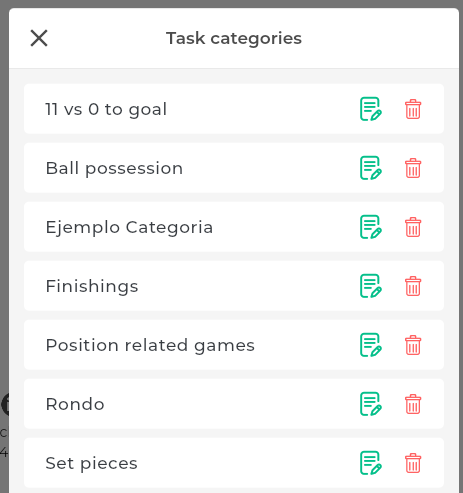
\includegraphics[width=10cm]{archivos/tfg_jorge/bcoach_kpis}
    \caption{Bcoach - Crear categoría de tarea}\label{sistemass2}
\end{figure}

\subsection{Football tactical Board}
Aplicación web gratuita con una gran variedad de deportes. Para fútbol, ofrece tres tipos de vista (Horizontal, Vertical y Medio campo). Ofrece únicamente una pizarra con figuras gráficas con la posibilidad de crear una ‘conferencia’ dónde es posible alojar a muchos usuarios que verán al mismo tiempo lo que está sucediendo en la pizarra.
Dispone de una versión Pro que elimina los anuncios y permite descargar y grabar las acciones con la pizarra.

\subsubsection{Manejo de estadísticas e indicadores de rendimiento}
Football Tactical Board es una herramienta principalmente enfocada en la creación de diagramas tácticos y la visualización de estrategias de juego. No está diseñada específicamente para la gestión y análisis de estadísticas avanzadas como los KPIs. Las funcionalidades ya nombradas permiten hacerse durante una conferencia en tiempo real, sin embargo, no aparece la opción sobre la creación de métricas.

\begin{figure}[H]
    \centering
    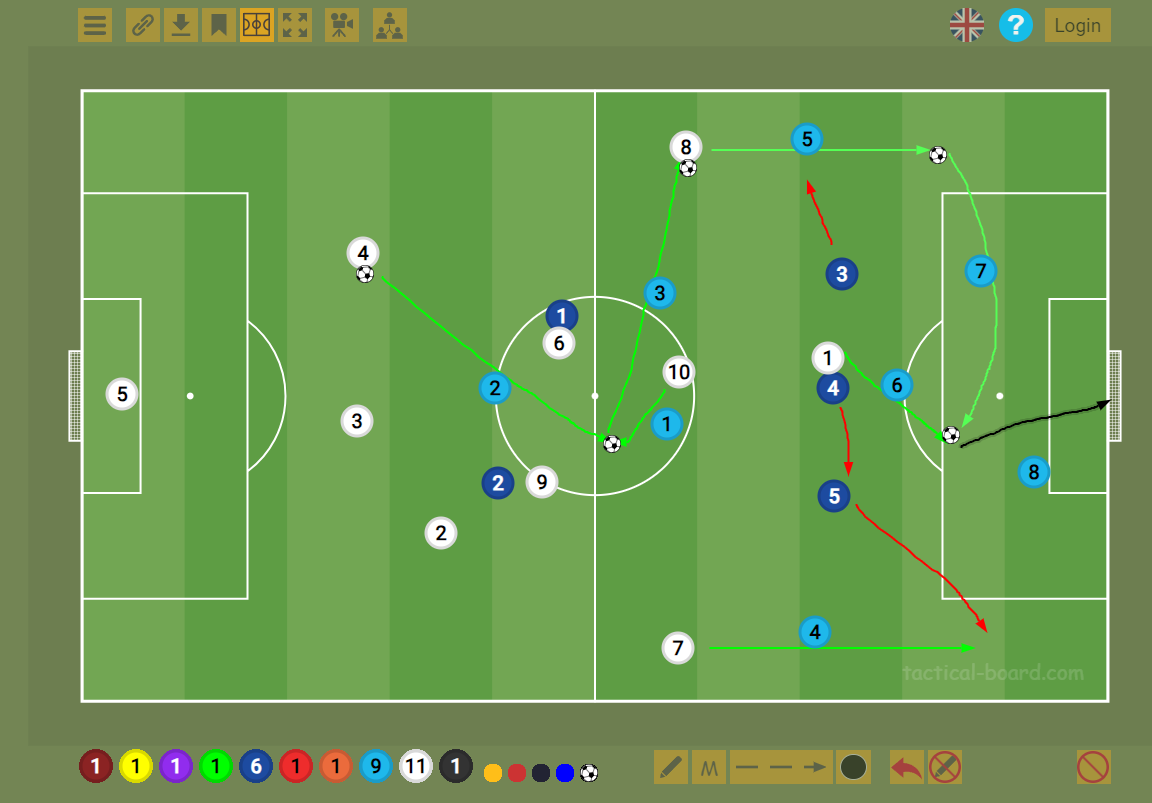
\includegraphics[width=10cm]{archivos/tfg_jorge/tbo_pizarra}
    \caption{Football Tactical Board - Pantalla del entrenador}\label{sistemass2}
\end{figure}


\subsection{Sportlyzer Players App}
Aplicación disponible tanto para Android como para IOS que ofrece opciones para entrenadores, clubes y padres

\subsubsection{Entrenadores}

\subparagraph{Horarios y Tareas}
Dispone de un calendario compartido entre todos los usuarios, cuándo el entrenador actualiza el calendario con un nuevo evento, todo el mundo podrá ver los cambios. El calendario ofrece las siguientes acciones:

\begin{itemize}
    \item Importar partidos y competiciones desde Excel
    \item Configurar entrenamientos regulares
    \item Compartir eventos por email
    \item Widget para mostrar el calendario en la web del club
    \item Anotar asistencia de los deportistas
    \item Asignación y seguimiento de deberes
\end{itemize}

\subparagraph{Disponibilidad}
Esta opción se usa para planificar actividades que necesitan mínimo de personas. Recoge información sobre qué deportistas asistirán o no a cada evento del calendario. Los enlaces son únicos para cada deportista, por lo que no necesitarán registrarse.

\subparagraph{Asistencia}
Anota la asistencia de los deportistas, pudiendo ser evaluada en un registro con el total de ausencias de cada uno, la anotación se puede hacer de forma offline.

\subparagraph{Retroalimentación}
Forma en la que los jugadores pueden comentar y valorar cada sesión, pueden dar una nota al entrenamiento, valorar cuán duro ha sido o simplemente dejar un comentario.

\subparagraph{Planificación y análisis}
Para ir desarrollando a los jugadores, la plataforma permite crear ciclos con planes de entrenamiento, pudiendo calibrar su intensidad. Después de cada uno se podrá recoger los comentarios y un análisis de los resultados.

\subparagraph{Evaluación y prueba de jugadores}
Seguimiento de cada jugador, evaluación de cada aptitud (física, táctica o técnica), personalidad y habilidades. Se puede enviar un informe de la evaluación a cada jugador. 

\subparagraph{Mensajería}
Permite enviar SMS o correos electrónicos a cada jugador y mantener conversaciones


\subsubsection{Clubes}

\subparagraph{Base de datos}
Es la manera para gestionar todos los miembros del club, en la base de datos se incluyen perfiles para deportistas, que rellenando un formulario de inscripción se crearán sus perfiles.

\subparagraph{Horarios y deberes de equipo}
Los clubes también pueden ver el calendario compartido por el entrenador y los jugadores.

\subparagraph{Facturas}
Enviar facturas a todo el club y hacer un seguimiento de los pagos, pudiendo enviar recordatorios a los impagados.

\subparagraph{Padres y Jugadores}
Este grupo de usuarios dispondrá de una app móvil donde tendrán acceso al horario de entrenamiento; mensajería con el entrenador; historial de asistencia; organizar desplazamientos a otros pares/jugadores y actualizar los detalles de contacto del jugador.


\subsubsection{Precios}
La aplicación ofrece precios mensuales o anuales (con un 30\% de descuento sobre el mensual) dependiendo del tamaño del club. La diferencia de precios escala con una diferencia de 7€ entre los tramos que van en grupos de 25 jugadores.

\subsubsection{Manejo de estadísticas e indicadores de rendimiento}
Aunque esta aplicación se enfoca en la gestión y mejora del rendimiento deportivo de los jugadores, ofrece algunas funcionalidades que pueden ser útiles para el análisis de indicadores de rendimiento. Pudiendo servir para su análisis, no se menciona en su documentación ni aparece de forma clara dentro de las interfaces ninguna opción para crear estos indicadores.

La aplicación ofrece precios mensuales o anuales (con un 30\% de descuento sobre el mensual) dependiendo del tamaño del club. La diferencia de precios escala con una diferencia de 7€ entre los tramos que van en grupos de 25 jugadores.

\begin{figure}[h]
    \centering
    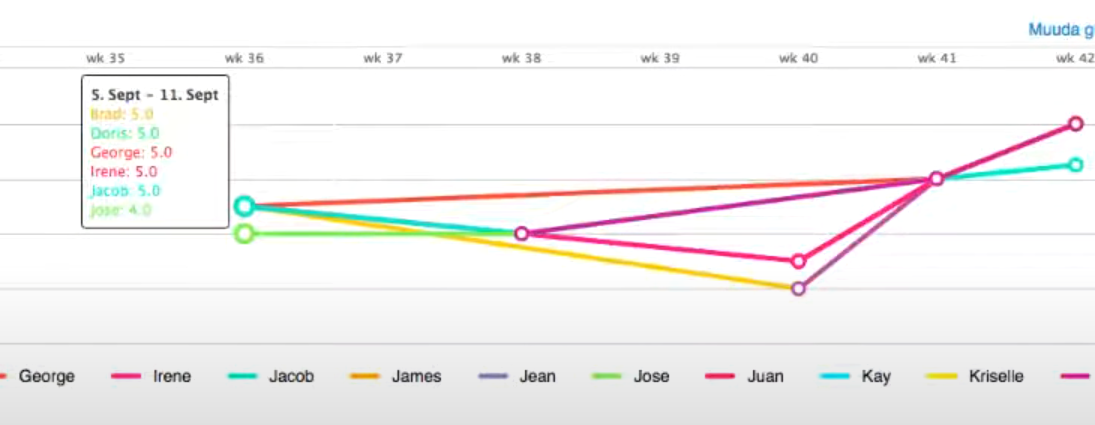
\includegraphics[width=10cm]{archivos/tfg_jorge/sportlyzer_graph_sesion_entrenamiento}
    \caption{Sportlyzer Players App - Gráfico de los tiempos de finalización del entrenamiento}\label{sistemass2}
\end{figure}


\subsection{LongoMatch}
Esta aplicación ofrece la retransmisión de partidos repetidos, con la posibilidad de dibujar sobre las imágenes de vídeo y colocar momentos importantes para ser analizados.
Ofrece dos planes diferentes:

\begin{itemize}
    \item 15€/mes o 150€/año: Proyectos ilimitados, equipos, paneles y eventos. Análisis en directo con múltiples cámaras y  administrador de base de datos.
    \item 55€/mes o 550€/año: Ofrece las posibilidades anteriores, junto con zoom durante el video, importar o exportar archivos XML y compatibilidad con otras herramientas.
\end{itemize}

\subsubsection{Manejo de estadísticas e indicadores de rendimiento}
Aunque LongoMatch no está específicamente diseñado para la creación de KPIs personalizados, se pueden crear plantillas de etiquetado que correspondan a los KPIs específicos que deseemos rastrear. Por ejemplo, puedes tener etiquetas para "Controles de Balón Exitosos", "Intercepciones", etc. Además, los informes generados por LongoMatch pueden incluir gráficos y estadísticas basadas en los eventos etiquetados, permitiendo una evaluación detallada de los KPIs.

\begin{figure}[H]
    \centering
    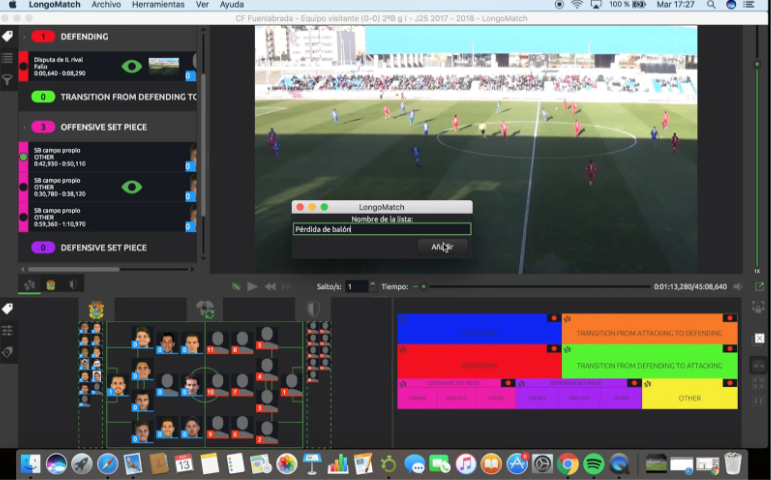
\includegraphics[width=10cm]{archivos/tfg_jorge/longomatch_eventos_live_video}
    \caption{Longomatch - Creación de eventos en el vídeo}\label{sistemass2}
\end{figure}

\subsection{Picco: Estadísticas y rendimiento}
Esta app es completamente gratis (con opción a pago para quitar anuncios) contiene una multitud de opciones para la recogida y el análisis de los datos. Durante el partido, el analista puede apuntar cada dato estadístico que él considere.
Esta pantalla de datos puede ser la más útil a la hora de recoger datos durante el partido, pues solo hay que  marcar cada registro a la vez que se va desarrollando el partido.

\subsubsection{Manejo de estadísticas e indicadores de rendimiento}
Picco es especialmente útil para la creación y seguimiento de KPIs debido a su capacidad de personalización y análisis detallado. Tiene la posibilidad de definir KPIs específicos , por ejemplo, puedes crear indicadores como "Tasa de éxito en pases", "Distancia recorrida por jugador", entre otros. Todos estos siendo recogidos y actualizados en tiempo real asegurando datos precisos y disponibilidad inmediata.

\begin{figure}[H]
    \centering
    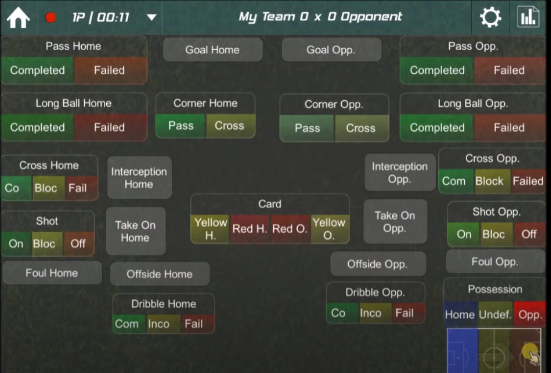
\includegraphics[width=10cm]{archivos/tfg_jorge/picco_ui_partidos}
    \caption{Picco - Interfaz durante el partido}\label{sistemass2}
\end{figure}

\subsection{Teamtag}
Esta aplicación es parecida a la Picco, teniendo funcionalidades más allá de los pocos paneles que contiene Picco, esta aplicación se enfoca en la gestión de un club, pudiendo crear eventos de partidos para ir apuntando las estadísticas a medida que transcurre el evento. Permite crear tus propios equipos y alineaciones para cuando un evento estadístico sea registrado, indicar que jugador/a lo ocasionó y en qué zona del campo ocurrió.

\subsubsection{Manejo de estadísticas e indicadores de rendimiento}
Al igual que la aplicación anterior, permite la definición de indicadores personalizados que se irán recogiendo en tiempo real.

\begin{figure}[H]
    \centering
    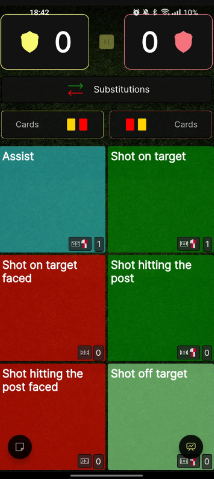
\includegraphics[width=3cm]{archivos/tfg_jorge/teamtag_movil_ui}
    \caption{Teamtag - Interfaz durante el partido}\label{sistemass2}
\end{figure}

\subsection{Conclusiones}
Una vez analizadas las aplicaciones del mercado, podemos concluir la función de cada una.
Bcoach:
\begin{itemize}
    \item Planificación de entrenamientos con animaciones.
    \item Pizarra táctica.
    \item Estadísticas de partidos.
    \item Planes desde 2,99€/mes.
\end{itemize}

Sportlyzer Players App:
\begin{itemize}
    \item Para entrenadores, clubes y jugadores.
    \item Horarios y tareas con calendario compartido.
    \item Asignación de deberes y seguimiento de asistencia.
    \item Evaluación y análisis de jugadores.
    \item Mensajería con jugadores.
    \item Planes desde 7€/mes por jugador.
\end{itemize}

LongoMatch:
\begin{itemize}
    \item Retransmisión de partidos repetidos.
    \item Dibujar sobre video y análisis de momentos importantes.
    \item Planes desde 15€/mes.
\end{itemize}

Picco y Teamtag:
\begin{itemize}
    \item Recogida y análisis de datos estadísticos.
    \item Gratis (con opción de pago para quitar anuncios).
\end{itemize}

Dependiendo de las necesidades, Bcoach o Sportlyzer podrían ser las más completas para la gestión de los equipos. Y si el problema es el presupuesto, Football Tactical Board o Picco podrían ser también buenas opciones

\subsubsection{Manejo de estadísticas e indicadores de rendimiento}
El manejo de estadísticas e indicadores de rendimiento es crucial para el análisis y la mejora continua del desempeño de los jugadores y equipos. Cada una de las aplicaciones analizadas ofrece diferentes niveles de soporte para estas funcionalidades:

\subparagraph{Bcoach}
\begin{itemize}
    \item Ofrece categorías de tarea que se relacionan directamente con los indicadores de rendimiento.
    \item Estadísticas que se modifican durante los partidos para analizar esas categorías.
\end{itemize}
\subparagraph{Football Tactical Board}
\begin{itemize}
    \item Enfocada en la creación de diagramas tácticos y estrategias de juego.
    \item No diseñada específicamente para la gestión y análisis de estadísticas avanzadas como los KPIs.
\end{itemize}

\subparagraph{Sportlyzer Players App}
\begin{itemize}
    \item Enfocada en la gestión y mejora del rendimiento deportivo.
    \item Funcionalidades útiles para el análisis de indicadores de rendimiento, aunque no ofrece una opción clara para la creación de KPIs.
\end{itemize}

\subparagraph{LongoMatch}
\begin{itemize}
    \item Permite etiquetar eventos específicos durante los partidos y analizarlos posteriormente.
    \item Informes generados pueden incluir gráficos y estadísticas basadas en los eventos etiquetados.
\end{itemize}

\subparagraph{Picco}
\begin{itemize}
    \item Especialmente útil para la creación y seguimiento de KPIs debido a su capacidad de personalización.
    \item Recogida y actualización de datos en tiempo real.
\end{itemize}

\subparagraph{Teamtag}
\begin{itemize}
    \item Permite la definición de indicadores personalizados que se irán recogiendo en tiempo real.
    \item Gestión de equipos y alineaciones, registro de eventos y análisis de datos.
\end{itemize}

En resumen, todas las aplicaciones analizadas ofrecen herramientas útiles para el manejo de estadísticas e indicadores de rendimiento, aunque no todas ofrecen la opción de crear indicadores personalizados.
\section{Tabla comparativa}

\begin{table}[ht]
{\tiny % Usar \tiny o \scriptsize para hacerlo aún más pequeño
\begin{tabular}{|m{14mm}|m{12mm}|m{14mm}|m{10mm}|m{14mm}|m{8mm}|m{14mm}|m{12mm}|m{10mm}|m{14mm}|}
\hline
\textbf{Aplicación} & \textbf{Estadísticas predefinidas} & \textbf{Creación de nuevas estadísticas} & \textbf{En tiempo real} & \textbf{Individuales} & \textbf{Grupales} & \textbf{Informe generado} & \textbf{Seguimiento contínuo} & \textbf{Toma de decisión} & \textbf{KPIs Personalizables} \\
\hline
Bcoach & \ding{51} & \ding{51} & \ding{51} & \ding{51} & \ding{51} & \ding{51} & \ding{51} & \ding{55} & \ding{51} \\
\hline
Sportlyzer Players App & \ding{51} & \ding{55} & \ding{55} & \ding{51} & \ding{51} & \ding{51} & \ding{51} & \ding{55} & \ding{55} \\
\hline
LongoMatch & \ding{55} & \ding{51} & \ding{51} & \ding{55} & \ding{51} & \ding{55} & \ding{55} & \ding{55} & \ding{55} \\
\hline
Picco & \ding{51} & \ding{51} & \ding{51} & \ding{55} & \ding{51} & \ding{55} & \ding{55} & \ding{55} & \ding{51} \\
\hline
Teamtag & \ding{51} & \ding{55} & \ding{51} & \ding{51} & \ding{51} & \ding{51} & \ding{51} & \ding{55} & \ding{51} \\
\hline
\end{tabular}
\caption{Comparativa de funcionalidades de aplicaciones} % Título de la tabla para el índice y visualización
\label{tab:comparativa_funcionalidades} % Etiqueta para referencias cruzadas
}
\end{table}

